\documentclass[conference]{IEEEtran}

\usepackage[T1]{fontenc}
\usepackage[utf8]{inputenc}
\usepackage{amsmath,amssymb}
\usepackage{booktabs}
\usepackage{graphicx}
\usepackage{microtype}
\usepackage{multirow}
\usepackage{url}
\usepackage{xspace}
\usepackage{xcolor}
\usepackage{tikz}
\usetikzlibrary{arrows.meta,positioning,shapes.geometric,fit}
\usepackage{pgfplots}
\usepackage{pgfplotstable}
\pgfplotsset{compat=1.18}
\usepackage[hidelinks]{hyperref}

\newcommand{\DerivedDeadlineMs}{20}
\newcommand{\DeadlineSafetyFactor}{1.25}
\newcommand{\ObservationsPerCell}{1000}
\newcommand{\RecoveryImprovement}{36.6\%}
\newcommand{\RecoveryOracleRatio}{1.63}
\newcommand{\RecoveryTunedRatio}{2.95}
\newcommand{\PolicyCpuP}{170.1}
\newcommand{\PolicyWallP}{177.2}
\newcommand{\PolicyPeakBytes}{3138}
\newcommand{\LinuxCommP}{8.05}
\newcommand{\RtCommP}{11.42}
\newcommand{\KernelOverhead}{3.76\%}
\newcommand{\VisualizationOverhead}{2.05\%}


\definecolor{qblue}{RGB}{34,92,150}
\definecolor{qorange}{RGB}{222,119,38}
\definecolor{qgreen}{RGB}{52,128,73}
\definecolor{qred}{RGB}{178,55,55}
\newcommand{\system}{QFabric\xspace}
\newcommand{\linuxdom}{Linux}
\newcommand{\rtdom}{RT}
\hypersetup{
  pdftitle={QFabric: Contract-Driven Recovery Across a Linux--RTOS Boundary},
  pdfauthor={Ayushman Bhattacharya},
  pdfsubject={Empirical soft real-time recovery across Linux and RTOS domains},
  pdfkeywords={heterogeneous embedded systems, Linux, RTOS, timing contracts}
}

\title{QFabric: Contract-Driven Recovery Across a Linux--RTOS Boundary}

\author{\IEEEauthorblockN{Ayushman Bhattacharya}
\IEEEauthorblockA{\href{mailto:ayushman@myceli.ai}{ayushman@myceli.ai}}}

\begin{document}
\maketitle

\begin{abstract}
Heterogeneous embedded boards increasingly combine an application processor
running Linux with a microcontroller running a real-time operating system.
Choosing one domain statically is simple, but timing behavior can change after
deployment, while unconstrained migration can violate program semantics or
overload the real-time domain. We present \system, a prototype that treats
placement as a closed-loop recovery problem for empirical soft real-time
contracts. It profiles the same bounded task in both domains, observes
end-to-end latency windows, rejects semantically or temporally inadmissible
moves, switches only at a quiescent epoch boundary, and commits or rolls back
after a probation window. On an Arduino UNO Q, a Linux--Zephyr platform, direct
measurements characterize communication, profiling, decision, and
instrumentation overheads. Deterministic replay of those measured traces over
four application graphs compares seven policies. In a four-node load-shift
case, ordinary Linux misses 67.3\% of 80-ms deadlines at a 111.30-ms p95;
\system recovery reduces p95 by \RecoveryImprovement to 70.61 ms and the miss
rate to 3.7\%. A tuned \texttt{SCHED\_FIFO} baseline remains substantially
better at 23.91 ms and zero misses. Thus, the result is not that adaptation
dominates expert tuning, but that bounded, semantics-aware recovery can salvage
an untuned deployment when its original contract stops holding. The complete
source, raw evidence, audits, and manuscript generators are released as a
reproducible artifact.
\end{abstract}

\begin{IEEEkeywords}
heterogeneous embedded systems, Linux, RTOS, runtime adaptation, timing
contracts, task migration, empirical evaluation
\end{IEEEkeywords}

\section{Introduction}
Modern embedded platforms often put two distinct execution environments on one
board: a feature-rich Linux application processor and a resource-constrained
real-time microcontroller. Linux offers libraries, networking, storage, and
developer velocity; the microcontroller offers isolation and more predictable
execution. A task that can execute in either domain therefore faces a placement
choice whose consequences extend beyond compute time: crossing the boundary
adds serialization and transport cost, contention changes tail latency, and a
move may be illegal for a stateful or Linux-only operation.

Classical heterogeneous schedulers optimize a static directed acyclic graph
from cost estimates~\cite{topcuoglu2002heft}. Real-time theory provides strong
admission and schedulability foundations~\cite{liu1973scheduling}, while
feedback scheduling adapts resources to measured error~\cite{lu2002feedback}.
Runtime verification and timing contracts make violations observable
\cite{reinbacher2014runtime,nandi2015contracts}. Yet an engineering gap remains
on asymmetric Linux--RTOS boards: how should a deployed task recover when an
empirical timing contract fails, without treating a faster prediction as
sufficient permission to migrate?

\system addresses that gap as a deliberately narrow systems contribution. A
portable QTask declaration is compiled for both domains. Offline measurements
seed placement and an empirical contract. At runtime, a monitor applies
hysteresis to complete observation windows. A recovery controller admits a
candidate only if its semantics, predicted end-to-end cost, real-time
utilization, evidence, and cooldown constraints all pass. It then drains
in-flight work, increments an epoch, switches, and evaluates a probation
window. The move is committed only if post-switch observations satisfy the
contract; otherwise it is rolled back.

This paper makes four contributions:

\begin{itemize}
  \item a cross-domain QTask interface with an explicitly bounded wire ABI and
  effect annotations used as migration constraints;
  \item a closed-loop recovery protocol combining empirical timing contracts,
  RT admission, quiescent epoch switching, and post-switch verification;
  \item an evidence chain that distinguishes direct hardware measurements from
  deterministic application-graph trace replay and machine-checks all reported
  claims; and
  \item an evaluation against ordinary Linux, tuned Linux, static and manual
  placements, a non-adaptive \system policy, recovery, and an offline oracle.
\end{itemize}

The central result is intentionally qualified. \system improves a failing
ordinary-Linux deployment, but it does not outperform correctly tuned Linux or
the oracle in our flagship case. This negative comparison clarifies where the
prototype is useful: recovery when prior deployment assumptions no longer hold,
not replacement of platform-specific real-time engineering.

\section{Platform and Problem}
\subsection{Target platform}
The Arduino UNO Q combines a quad-core Arm Cortex-A53 application processor
running Debian Linux with an STM32U585 Cortex-M33 microcontroller running
Zephyr~\cite{arduinoUnoQ}. Arduino's Bridge stack exposes MessagePack remote
procedure calls in both directions~\cite{arduinoRouterBridge}. Its underlying
architecture is representative of remote-processor systems built around
\texttt{remoteproc} and \texttt{rpmsg} abstractions
\cite{linuxRemoteproc,linuxRpmsg}, but our implementation targets the stock UNO
Q software stack rather than modifying the transport.

\begin{figure*}[t]
\centering
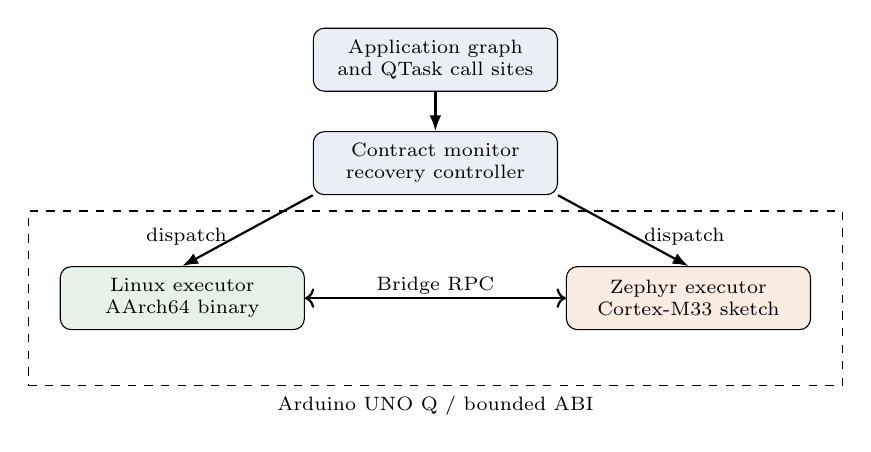
\begin{tikzpicture}[
  font=\scriptsize,
  node distance=5mm and 8mm,
  box/.style={draw,rounded corners,minimum width=31mm,minimum height=8mm,align=center},
  flow/.style={-{Latex[length=2mm]},thick}
]
\node[box,fill=qblue!10] (app) {Application graph\\and QTask call sites};
\node[box,fill=qblue!10,below=of app] (ctl) {Contract monitor\\recovery controller};
\node[box,fill=qgreen!12,below left=9mm and 1mm of ctl] (linux) {Linux executor\\AArch64 binary};
\node[box,fill=qorange!14,below right=9mm and 1mm of ctl] (rt) {Zephyr executor\\Cortex-M33 sketch};
\draw[flow] (app) -- (ctl);
\draw[flow] (ctl.south west) -- node[left,pos=0.58]{dispatch} (linux.north);
\draw[flow] (ctl.south east) -- node[right,pos=0.58]{dispatch} (rt.north);
\draw[flow,<->] (linux) -- node[above,fill=white,inner sep=1pt]{Bridge RPC} (rt);
\node[draw,dashed,fit=(linux)(rt),inner xsep=4mm,inner ysep=7mm,
      label={[font=\scriptsize]below:{Arduino UNO Q / bounded ABI}}] {};
\end{tikzpicture}
\caption{\system architecture. The policy runs in Linux userspace; task code
has a native implementation in each domain.}
\label{fig:architecture}
\end{figure*}

\subsection{System model}
An application is a directed graph $G=(V,E)$. Each task $t\in V$ may have a
Linux implementation, an RT implementation, or both. Its declaration includes
fixed-width request and response types, a numeric task identifier, and an
effect class. In this prototype, only pure, bounded tasks are migration
eligible. Each edge $e\in E$ incurs a measured boundary cost $b_e$ when its
endpoints occupy different domains.

For task $t$ in domain $d$, profiling yields a latency distribution and its
empirical 95th percentile $q_{.95}(t,d)$. Given neighboring placements, the
policy estimates
\begin{equation}
 \widehat C(t,d)=q_{.95}(t,d)+
 \sum_{e\in E_t}\mathbf{1}[d\ne d_{\mathrm{neighbor}(e)}]b_e .
 \label{eq:cost}
\end{equation}
This is a transparent heuristic, not a worst-case execution-time proof. The
contract deadline $D$ and tolerated miss rate $\epsilon$ likewise describe an
empirical soft real-time objective.

For a complete window $w$ of $n$ observations with outcome $o_i$ and latency
$L_i$, the observed miss rate is
\begin{equation}
 \widehat m_w=\frac{1}{n}\sum_{i=1}^{n}
 \mathbf{1}[o_i\ne\mathrm{ok}\ \lor\ L_i>D].
 \label{eq:miss}
\end{equation}
A violation means $\widehat m_w>\epsilon$. Consecutive-window thresholds avoid
reacting to a single outlier.

\subsection{Research questions}
The evaluation asks: \textbf{RQ1}, can the controller detect a sustained
contract failure without false switches? \textbf{RQ2}, can a feasible switch
improve the violated contract? \textbf{RQ3}, are unsafe or unsupported switches
rejected? \textbf{RQ4}, how does recovery compare with deployable baselines and
an oracle? \textbf{RQ5}, what overheads does the mechanism introduce? and
\textbf{RQ6}, what programmer effort is visible in the prototype?

\section{Related Work}
HEFT ranks a task graph and maps tasks to heterogeneous processors using
estimated computation and communication costs~\cite{topcuoglu2002heft}. It is a
natural static-placement reference, but it does not monitor deployed timing
contracts. Feedback real-time scheduling instead adjusts resource allocation
from runtime error~\cite{lu2002feedback}; autonomic computing generalizes the
monitor--analyze--plan--execute loop~\cite{kephart2003autonomic}. \system uses a
feedback loop, but its actuator is a guarded cross-domain implementation switch.

Runtime verification can observe real-time behavior with bounded intrusion
\cite{reinbacher2014runtime}. Stochastic contracts provide empirical runtime
checks for component systems~\cite{nandi2015contracts}, while formal timing
contracts and zone-based models support verification and synthesis
\cite{alkhatib2016timing,camilli2018adaptive}. These works motivate contract
semantics; our focus is the operational recovery protocol after a violation.

Real-time task migration has been studied for dynamic resource management in
many-core systems with feasibility analysis~\cite{pourmohseni2020migration}.
Linux also supplies deadline-aware scheduling mechanisms
\cite{lelli2016deadline}. \system does not replace either: it combines a simple
RT utilization guard with empirical cross-domain evidence, and explicitly
compares against tuned Linux scheduling.

Table~\ref{tab:related} locates the contribution. A checkmark means the feature
is central to the cited work, not that it could not be added. To the best of
our literature search, the combined column pattern---empirical violation,
semantic guard, RT admission, atomic switch, and post-switch verification on a
physical Linux--RTOS boundary---is the distinctive part of \system. We do not
claim novelty for heterogeneous placement, profiling, feedback control, or
timing contracts individually.

\begin{table*}[t]
\caption{Qualitative positioning against representative prior work}
\label{tab:related}
\centering
\scriptsize
\setlength{\tabcolsep}{3.2pt}
\begin{tabular}{lcccccc}
\toprule
Work & Heterogeneous placement & Empirical monitor & Semantic guard & RT admission & Verified switch & Linux--RTOS board \\
\midrule
HEFT~\cite{topcuoglu2002heft} & \checkmark & -- & -- & -- & -- & -- \\
Feedback scheduling~\cite{lu2002feedback} & -- & \checkmark & -- & model-specific & -- & -- \\
Stochastic contracts~\cite{nandi2015contracts} & -- & \checkmark & -- & -- & -- & -- \\
RT task migration~\cite{pourmohseni2020migration} & \checkmark & -- & -- & \checkmark & migration protocol & -- \\
Bridge / rpmsg~\cite{arduinoRouterBridge,linuxRpmsg} & transport only & -- & -- & -- & -- & \checkmark \\
\system & \checkmark & \checkmark & \checkmark & \checkmark & \checkmark & \checkmark \\
\bottomrule
\end{tabular}
\end{table*}

\section{QFabric Design}
\subsection{QTask declaration and bounded ABI}
A QTask declaration is the single source for Linux and MCU artifacts. The
generator accepts fixed-size scalars, records, and bounded arrays; it rejects
pointers, dynamic arrays, recursive types, unsupported effects, and messages
larger than the 988-byte payload budget. Versioned big-endian headers carry a
magic value, message kind, task identifier, request identifier, payload length,
and flags. Golden vectors are checked independently in Python, C++, and on the
MCU. These restrictions turn serialization bounds and effect eligibility into
auditable facts rather than conventions.

The current prototype exposes one concrete task, integer addition. That task is
purposefully small: it isolates placement and communication behavior, but it
also limits external validity. Section~\ref{sec:threats} treats this directly.

\subsection{Contracts and admission}
The profiler measures both implementations using warm-up exclusion and retains
raw observations. A minimum sample count marks an estimator valid; cold-start
runs remain labeled insufficient rather than silently promoted to evidence.
The prototype derives its per-node deadline before application replay:
\begin{equation}
 D=\left\lceil 1.25\max_r p99_r\right\rceil_{5\,\mathrm{ms}}
   = \DerivedDeadlineMs\,\mathrm{ms},
 \label{eq:deadline}
\end{equation}
where $p99_r$ are three idle round-trip repetitions. The derivation is recorded
as non-post-hoc in the artifact.

A candidate RT move must leave utilization beneath a reserved headroom $h$:
\begin{equation}
 U'_{RT}=U_{RT}+r_t\,q_{.95}(t,RT)\le 1-h,
 \label{eq:admission}
\end{equation}
where $r_t$ is the invocation rate. A switch is admissible only when
\begin{align}
 A(t,d)={}&E_{\min}\land S_{\mathrm{semantic}}\land
 S_{\mathrm{admission}} \notag\\
 &\land (\widehat C(t,d)\le D)\land S_{\mathrm{cooldown}}.
 \label{eq:admissible}
\end{align}
The controller reports a stable rejection code for every failed conjunct.

\subsection{Safe recovery protocol}
Figure~\ref{fig:state} shows the recovery state machine. Three consecutive
violating windows trigger analysis. If no candidate is admissible, placement is
unchanged. Otherwise the dispatcher stops accepting new work, waits until the
in-flight count is zero, increments a routing epoch, and changes the active
domain. Six probation windows then provide post-switch evidence. Satisfaction
commits the move; renewed violation rolls it back to the previous epoch and
domain. The protocol therefore distinguishes a predicted improvement from a
verified recovery.

\begin{figure}[t]
\centering
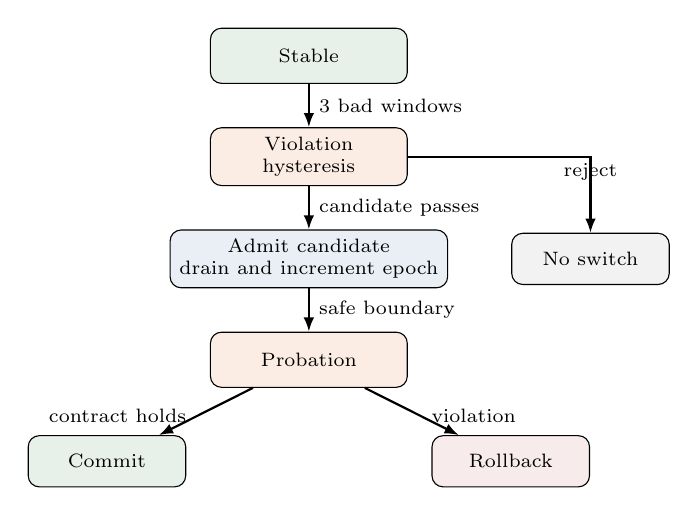
\begin{tikzpicture}[
  font=\scriptsize,
  node distance=5.5mm and 8mm,
  state/.style={draw,rounded corners,minimum width=25mm,minimum height=7mm,align=center},
  outcome/.style={draw,rounded corners,minimum width=20mm,minimum height=6.5mm,align=center},
  arr/.style={-{Latex[length=1.8mm]},thick}
]
\node[state,fill=qgreen!12] (stable) {Stable};
\node[state,fill=qorange!13,below=of stable] (viol) {Violation\\hysteresis};
\node[state,fill=qblue!10,below=of viol] (drain) {Admit candidate\\drain and increment epoch};
\node[outcome,fill=gray!10,right=of drain] (noswitch) {No switch};
\node[state,fill=qorange!13,below=of drain] (prob) {Probation};
\node[outcome,fill=qgreen!12,below left=6mm and 3mm of prob] (commit) {Commit};
\node[outcome,fill=qred!10,below right=6mm and 3mm of prob] (rollback) {Rollback};
\draw[arr] (stable) -- node[right,pos=0.5]{3 bad windows} (viol);
\draw[arr] (viol) -- node[right,pos=0.5]{candidate passes} (drain);
\draw[arr] (viol.east) -| node[above,pos=0.72]{reject} (noswitch.north);
\draw[arr] (drain) -- node[right,pos=0.5]{safe boundary} (prob);
\draw[arr] (prob) -- node[left,pos=0.6]{contract holds} (commit);
\draw[arr] (prob) -- node[right,pos=0.6]{violation} (rollback);
\end{tikzpicture}
\caption{Contract recovery. Prediction authorizes probation, not commitment;
each terminal outcome returns the monitor to Stable.}
\label{fig:state}
\end{figure}

\section{Implementation}
The implementation comprises a Python command-line controller and evidence
pipeline, generated C++ ABI code, an AArch64 Linux executor, and Arduino/Zephyr
sketches. The policy executes in Linux userspace. Bridge RPC carries task calls
and diagnostics; the stock router remains responsible for transport. A
resource probe reports compile-time capacities and explicitly marks runtime
heap and stack statistics unavailable when the stock firmware cannot expose
them safely.

Instrumentation is layered. Reduced mode records core timing; full mode adds
structured observations; disabled mode measures the base call path. An optional
kernel probe is evaluated separately and is not required for control. LED matrix
updates have disabled, static, and 10/30/60-Hz refresh profiles, making the
visual status display an experimentally bounded feature rather than unmeasured
decoration. All records carry schema versions, run identifiers, monotonic
timestamps, outcomes, payload sizes, and relevant mode metadata.

The artifact~\cite{qfabric2026} includes command-line audits for each development
stage. The final audit cross-checks source hashes, sample counts, baseline
coverage, derived deadlines, negative safety scenarios, direct hardware
recovery and rollback reports, graph outputs, and headline numbers.

\section{Evaluation Methodology}
\subsection{Testbed and evidence classes}
Table~\ref{tab:testbed} summarizes the setup. Measurements were collected on a
single UNO Q using its stock Linux--Zephyr Bridge. Performance campaigns fix the
Linux CPU governor during a run and restore it afterward. Loaded campaigns use
controlled CPU contention. Each main evaluation cell retains
\ObservationsPerCell observations with a fixed recorded seed.

\begin{table}[t]
\caption{Experimental setup}
\label{tab:testbed}
\centering
\small
\begin{tabular}{ll}
\toprule
Item & Configuration \\
\midrule
Board & Arduino UNO Q \\
Linux domain & Arm Cortex-A53, Debian, AArch64 \\
RT domain & STM32U585 Cortex-M33, Zephyr \\
Transport & Arduino Bridge RPC / MessagePack \\
Task & Bounded signed 32-bit integer addition \\
Per-cell evidence & \ObservationsPerCell observations \\
Per-node deadline & \DerivedDeadlineMs ms, pre-derived \\
Policy location & Linux userspace \\
Claim class & Empirical soft real-time \\
\bottomrule
\end{tabular}
\end{table}

\begin{figure}[t]
\centering
\IfFileExists{figures/testbed.jpg}{%
  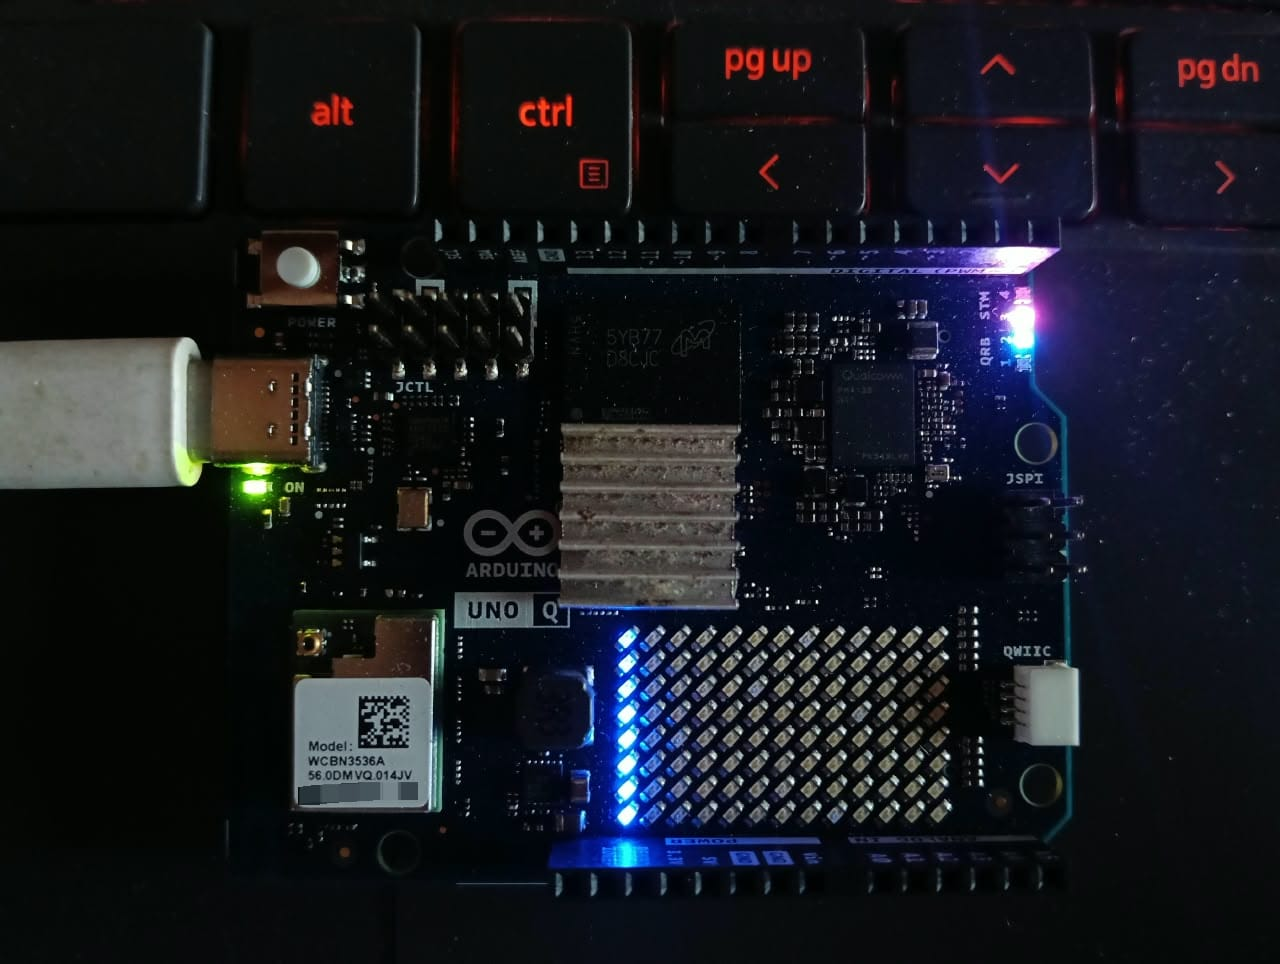
\includegraphics[width=\columnwidth]{figures/testbed.jpg}%
}{%
  \fbox{\parbox[c][32mm][c]{0.92\columnwidth}{\centering
  Testbed photograph pending\\[2mm]
  Add \texttt{paper/figures/testbed.jpg}; see capture instructions.}}%
}
\IfFileExists{figures/testbed.jpg}{%
\caption{Physical testbed displaying audited decision 2: an accepted
Linux-to-RT transition. Matrix rows encode the Linux source, RPC boundary, and
RT destination; the single illuminated column is the prototype's one QTask.}%
}{%
\caption{Testbed photograph placeholder. The intended capture is audited
decision 2, an accepted Linux-to-RT transition; no synthetic image is used.}%
}
\label{fig:testbed-photo}
\end{figure}

We keep three evidence classes separate. \emph{Direct measurements} are timing
observations produced on the board. \emph{Hardware scenarios} exercise the real
controller and demonstrate one successful commit and one rollback. Finally,
\emph{measured-trace replay} composes sampled board traces according to a fixed
application graph, placement, edge cost, and seed. Replay permits paired,
repeatable comparison across seven policies, but it is not equivalent to
running four complete application binaries.

\subsection{Applications and baselines}
The four models are a four-node synthetic chain, a three-node signal pipeline,
a three-node control loop, and a three-node network pipeline. Nodes differ in
semantic eligibility, including Linux-only operations. The flagship scenario
is the four-node chain under a Linux load shift with an 80-ms graph deadline.

We compare: (1) ordinary Linux; (2) Linux under \texttt{SCHED\_FIFO}; (3) a
static MCU-first rule; (4) a declared manual-expert placement; (5) \system's
static recommendation; (6) \system with recovery; and (7) an offline oracle
that chooses with future trace knowledge. The oracle is a lower-bound reference,
not a deployable competitor. Table~\ref{tab:baselines} makes the information
advantage explicit.

\begin{table}[t]
\caption{Baseline roles and information}
\label{tab:baselines}
\centering
\small
\begin{tabular}{lp{3.8cm}}
\toprule
Baseline & Role \\
\midrule
Ordinary Linux & Default deployment, no RT tuning \\
Tuned Linux & Deployable expert scheduler configuration \\
MCU-first & Static preference for eligible RT nodes \\
Manual expert & Declared per-graph hand placement \\
\system static & Profile-driven, no online recovery \\
\system recovery & Causal monitor and guarded switch \\
Offline oracle & Non-causal future-trace lower bound \\
\bottomrule
\end{tabular}
\end{table}

\subsection{Metrics and audit}
Primary metrics are end-to-end p95 latency and deadline-miss rate. We also
report detection and verification delay in complete windows, false switches,
rejection coverage, decision cost, traced Python allocation peak,
communication latency, profiling perturbation, kernel-probe overhead, and LED
visualization overhead. All percentile calculations and figures originate from
machine-readable data. The generator records the source SHA-256 in a manifest.

\section{Results}
\subsection{RQ1--RQ3: detection, recovery, and safety}
In the controlled hardware scenario, the sustained violation was detected one
complete window after onset, with zero false switches. A feasible alternate
was switched, observed, and verified after four windows. A separate injected
scenario forced probation failure and produced a rollback. The negative suite
exercised nine stable rejection reasons: insufficient evidence, unsatisfied
contract, semantic ineligibility, destination admission failure, MCU headroom,
predicted deadline miss, higher predicted end-to-end cost, observed miss-rate
failure, and active cooldown. These are bounded scenario results, not a proof
that all failures are impossible.

\subsection{RQ4: comparative effectiveness}
Table~\ref{tab:flagship} and Fig.~\ref{fig:flagship} give the central comparison.
Ordinary Linux and the static \system recommendation have identical failing
behavior because both keep all four nodes in Linux. Recovery shifts eligible
work and reduces p95 from 111.30 to 70.61 ms (\RecoveryImprovement), reducing
misses from 67.3\% to 3.7\%. The offline oracle places all nodes in RT and
achieves 43.45 ms with no misses.

The strongest deployable baseline is tuned Linux: 23.91 ms with no deadline
misses. Recovery is \RecoveryTunedRatio$\times$ its p95 and
\RecoveryOracleRatio$\times$ the oracle's. The tuned result is not an anomaly to
discard; it is the main boundary on our claim. If the workload can remain in
Linux and the deployment can be correctly configured, scheduler tuning is both
simpler and faster in this experiment. \system is valuable when the original
placement is already deployed, its empirical contract degrades, and a tested
alternate is available.

\begin{table*}[t]
\caption{Flagship four-node load-shift result. L denotes Linux and R denotes RT;
recovery and oracle placements vary over the trace.}
\label{tab:flagship}
\centering
\begin{tabular}{lrrr}
\toprule
Baseline & p95 (ms) & Miss rate (\%) & Placement \\
\midrule
ordinary-linux & 111.30 & 67.3 & L/L/L/L \\
tuned-linux & 23.91 & 0.0 & L/L/L/L \\
static-mcu-first & 43.45 & 0.0 & R/R/R/R \\
manual-expert & 100.93 & 58.3 & L/R/R/L \\
qfabric-static & 111.30 & 67.3 & L/L/L/L \\
qfabric-recovery & 70.61 & 3.7 & adaptive \\
offline-oracle & 43.45 & 0.0 & per observation \\
\bottomrule
\end{tabular}

\end{table*}

\begin{figure*}[t]
\centering
\pgfplotstableread{generated/flagship.dat}\flagshipdata
\begin{minipage}{0.49\textwidth}
\centering
\begin{tikzpicture}
\begin{axis}[
  ybar, width=\linewidth, height=48mm,
  ylabel={p95 latency (ms)}, ymin=0,
  symbolic x coords={ordinary-linux,tuned-linux,static-mcu-first,manual-expert,qfabric-static,qfabric-recovery,offline-oracle},
  xtick=data, x tick label style={rotate=38,anchor=east,font=\scriptsize},
  nodes near coords, nodes near coords style={font=\tiny,rotate=90,anchor=west},
  bar width=7pt, enlarge x limits=0.08, grid=major,
]
\addplot[fill=qblue!70,draw=qblue] table[x=baseline,y=p95_ms]{\flagshipdata};
\end{axis}
\end{tikzpicture}
\end{minipage}
\begin{minipage}{0.49\textwidth}
\centering
\begin{tikzpicture}
\begin{axis}[
  ybar, width=\linewidth, height=48mm,
  ylabel={Deadline-miss rate (\%)}, ymin=0,ymax=75,
  symbolic x coords={ordinary-linux,tuned-linux,static-mcu-first,manual-expert,qfabric-static,qfabric-recovery,offline-oracle},
  xtick=data, x tick label style={rotate=38,anchor=east,font=\scriptsize},
  nodes near coords, nodes near coords style={font=\tiny},
  bar width=7pt, enlarge x limits=0.08, grid=major,
]
\addplot[fill=qorange!75,draw=qorange] table[x=baseline,y=miss_rate_pct]{\flagshipdata};
\end{axis}
\end{tikzpicture}
\end{minipage}
\caption{Flagship end-to-end result from deterministic replay of measured board
traces. The graph deadline is 80 ms.}
\label{fig:flagship}
\end{figure*}

Under idle traces, the selected static placement does not improve all-Linux
execution for these small tasks. For example, the synthetic chain has a
31.72-ms all-Linux p95, while MCU-first reaches 43.53 ms and the declared manual
placement 56.04 ms. Boundary and RT invocation costs dominate the trivial
addition kernel. This reinforces why movement is a recovery action rather than
a universal optimization.

\subsection{RQ5: overhead}
Table~\ref{tab:overhead} reports measured overhead components. One policy
decision costs \PolicyCpuP\,$\mu$s CPU time and \PolicyWallP\,$\mu$s wall time
at p95 over 1,000 in-process evaluations, with a \PolicyPeakBytes-byte peak
observed by \texttt{tracemalloc}. That memory value excludes the interpreter
baseline and native allocator, so it is not total process memory.

Communication dominates policy cost: p95 is \LinuxCommP\,ms for the Linux path
and \RtCommP\,ms for the RT path. Full profiling changes Linux p95 by $-2.41$\%
and RT p95 by $+1.39$\% relative to disabled mode; the negative Linux delta is
measurement variation, not a speedup claim. Optional kernel instrumentation
adds \KernelOverhead at p95. The worst LED visualization delta is
\VisualizationOverhead. These results support userspace control at the tested
rate, but not arbitrary high-frequency control.

\begin{table}[t]
\caption{Measured mechanism costs}
\label{tab:overhead}
\centering
\small
\begin{tabular}{lr}
\toprule
Component & Result \\
\midrule
Policy CPU time, p95 & \PolicyCpuP\,$\mu$s \\
Policy wall time, p95 & \PolicyWallP\,$\mu$s \\
Policy traced peak & \PolicyPeakBytes\ bytes \\
Linux communication, p95 & \LinuxCommP\ ms \\
RT communication, p95 & \RtCommP\ ms \\
Full profiling delta, Linux & $-2.41$\% \\
Full profiling delta, RT & $+1.39$\% \\
Optional kernel probe delta & \KernelOverhead \\
Worst LED display delta & \VisualizationOverhead \\
\bottomrule
\end{tabular}
\end{table}

\subsection{RQ6: programmer effort}
The visible task declaration is a compact header that specifies types, effect,
and task identifier once. The generated ABI and common command-line workflow
remove hand-written marshaling from application code. However, the programmer
must still supply semantically equivalent Linux and RT implementations, choose
a defensible contract, and state any Linux-only effects. \system shifts effort
from transport plumbing toward explicit contracts and equivalence; it does not
eliminate dual-domain implementation or validation.

\begin{table}[t]
\caption{Answers to the research questions}
\label{tab:rq}
\centering
\small
\begin{tabular}{lp{5.7cm}}
\toprule
RQ & Audited answer \\
\midrule
RQ1 & Yes, with one-window detection in the controlled scenario and no false switch. \\
RQ2 & Yes for the tested feasible alternate; p95 improved \RecoveryImprovement. \\
RQ3 & Yes for nine enumerated negative scenarios plus hardware rollback. \\
RQ4 & Better than ordinary Linux, but worse than tuned Linux and the oracle. \\
RQ5 & Policy, transport, profiling, kernel, stabilization, and display costs quantified. \\
RQ6 & Declaration and generated ABI reduce plumbing; dual implementations remain required. \\
\bottomrule
\end{tabular}
\end{table}

\section{Discussion}
The experiment exposes three practical lessons. First, cross-domain placement
must include communication. The addition kernel is so small that Bridge cost
dominates, making static migration unattractive under idle conditions. Second,
recovery and tuning solve different problems. Tuned Linux is the right answer
when it can be applied reliably; contract recovery is a fallback when observed
behavior invalidates the current deployment. Third, a predicted faster domain
is not sufficient. Semantic eligibility, capacity admission, quiescence, and
post-switch verification are necessary to make adaptive placement operationally
credible.

The LED matrix is intentionally peripheral to the novelty. It exposes coarse
controller state for a physical demonstration, and its refresh cost is measured,
but it does not participate in scheduling decisions. This keeps presentation
quality from distorting the research claim.

\subsection{Threats to validity and limitations}
\label{sec:threats}
\textbf{External validity.} Results come from one UNO Q, one software stack,
one concrete QTask, and a single board instance. Other heterogeneous boards,
transports, kernels, thermal regimes, or workloads may reverse placement costs.
The application study replays measured traces over models; full applications
were not deployed end to end.

\textbf{Construct validity.} Empirical p95/p99 and miss rates do not establish
worst-case execution time or hard real-time guarantees. The RT admission test
is a conservative utilization gate, not a complete schedulability proof. MCU
runtime heap and stack watermarks were unavailable on stock firmware and are
reported as such rather than inferred.

\textbf{Internal validity.} Measurements share a board and may be affected by
uncontrolled firmware, caching, temperature, and OS activity. Fixed seeds and
paired trace replay improve repeatability but can underrepresent live
interactions. The deadline is derived before replay from Stage 1 data, which
reduces post-hoc bias but does not make it application-specific.

\textbf{Baseline validity.} \texttt{SCHED\_FIFO} is a strong but not exhaustive
Linux baseline; \texttt{SCHED\_DEADLINE}, CPU isolation, affinity, and kernel
tuning warrant future comparison. The manual baseline depends on the declared
expert mapping, while the oracle has non-causal information. We report both
roles explicitly.

\textbf{Safety scope.} Quiescent switching prevents mixed-epoch calls in the
prototype, and effect annotations reject known-ineligible tasks. This is not a
formal proof of implementation equivalence. Production use would require
stronger state-transfer semantics, authentication, fault containment, and
multi-client concurrency analysis.

\section{Artifact and Reproducibility}
The public repository~\cite{qfabric2026} contains source, generated code, unit
tests, board sketches, raw and processed results, campaign logs, negative
fixtures, SVG outputs, and stage audits. The final evaluation JSON is the source
of truth for this manuscript's quantitative macros, Table~\ref{tab:flagship},
and Fig.~\ref{fig:flagship}. Running
\texttt{make} in the \texttt{paper} directory first regenerates those assets,
records the input digest, and then builds the PDF. A real testbed photograph can
be added without changing the manuscript source; until then a visible
placeholder prevents a stock or synthetic image from being mistaken for
experimental evidence.

For archival citation, the repository is released as \texttt{v0.1.0} and is
prepared for deposition in a DOI-issuing archive. The release retains the
audited Stage 11 evidence used to generate this manuscript's results.

\section{Conclusion}
\system demonstrates a narrow but useful form of runtime adaptation across a
Linux--RTOS boundary: empirical contract violations initiate a guarded,
quiescent switch whose benefit must be observed before commitment. On one UNO Q
testbed, the mechanism detects controlled degradation, rejects enumerated unsafe
moves, commits a feasible recovery, and rolls back a failed one. Measured-trace
replay shows that recovery cuts flagship p95 by \RecoveryImprovement relative
to failing ordinary Linux, but remains almost \RecoveryTunedRatio$\times$ slower
than tuned Linux. That result defines the contribution honestly. QFabric is not
a universal scheduler or a hard-real-time proof; it is an auditable recovery
layer for deployments whose original empirical timing assumptions can cease to
hold. Broader tasks, boards, live application graphs, and stronger Linux
baselines are the next tests of generality.

\bibliographystyle{IEEEtran}
\bibliography{references}

\end{document}
